
\section{Descriptions des besoins}

\subsection{Besoins Fonctionnels}
\subsubsection{Plateau de Jeu}

\begin{center}
    \centering
    \begin{tabular}[h]{|m{14cm}|m{2cm}|}
        \hline
        \rowcolor[HTML]{FFA8A8}
        \multicolumn{2}{|c|}{\textbf{Priorité 3/3}}                                                                                                                  \\
        \hline
        Besoins                                                                                                                                         & Avancement \\
        \hline
        • Les hexagones numérotés, chacun représentant une distance définie, par défaut : 16 kilomètres                                                 & \FAIT      \\
        • Définir les joueurs et leurs spécificités. Par exemple les nationalités possibles, le joueur qui joue le premier et celui qui a l’initiative. & \FAIT      \\
        • Pouvoir poser des unités sur la carte et à retenir celles qui ne sont pas présentes dans celles-ci                                            & \FAIT      \\
        • Pouvoir poser plusieurs unités sur un hexagone                                                                                                & \FAIT      \\
        • Définir une séquence de tour :
        \begin{itemize}
            \item Pouvoir alterner entre les joueurs
            \item Respecter l’ordre strict d’un tour
        \end{itemize}
                                                                                                                                                        & \FAIT      \\
        • Afficher un terminal qui permettra aux joueurs de donner des commandes d'attaque ou mouvement                                                 & \FAIT      \\
        • Être capable de faire des lancés de dés et d’appliquer des modificateurs. La majeure partie du jeu se base sur les dés                        & \FAIT      \\
        • Pouvoir déterminer quel joueur a l’initiative                                                                                                 & \NOP       \\
        \hline
    \end{tabular}
\end{center}

\begin{center}
    \centering
    \begin{tabular}[h]{|m{14cm}|m{2cm}|}
        \hline
        \rowcolor[HTML]{FFB72B}
        \multicolumn{2}{|c|}{\textbf{Priorité 2/3}}                                                                                                                                           \\
        \hline
        Besoins                                                                                                                                                                  & Avancement \\
        \hline
        • Différencier plusieurs types de terrain, les montages, les mers de sable et les crêtes par exemple                                                                     & \FAIT      \\
        • Créer une base pour les cartes d’évènements. Celles-ci étant très différentes, l’implémentation sera limitée aux évènements génériques (non spécifiques aux scénarios) & \NOP       \\
        • Pouvoir charger la carte du jeu à partir d’un fichier \textsc{txt} ou \textsc{json} et pouvoir la sauvegarder aux mêmes formats                                        & \FAIT      \\
        \hline
    \end{tabular}
\end{center}

\begin{center}
    \centering
    \begin{tabular}[h]{|m{14cm}|m{2cm}|}
        \hline
        \rowcolor[HTML]{C0D8C0}
        \multicolumn{2}{|c|}{\textbf{Priorité 1/3}}                                                                                  \\
        \hline
        Besoins                                                                                                         & Avancement \\
        \hline
        • Ajouter les différents types d’indicateurs afin d’illustrer les villages, les villes et les oasis par exemple & \FAIT      \\
        \hline
    \end{tabular}
\end{center}

\subsubsection{API}

\begin{center}
    \centering
    \begin{tabular}[h]{|m{14cm}|m{2cm}|}
        \hline
        \rowcolor[HTML]{FFA8A8}
        \multicolumn{2}{|c|}{\textbf{Priorité 3/3}}                                                                                               \\
        \hline
        Besoins                                                                                                                      & Avancement \\
        \hline
        • Pouvoir échanger des informations basiques entre serveur et client                                                         & \FAIT      \\
        • Pouvoir convertir un état de la carte du jeu en format utilisable par le client pour pouvoir ensuite afficher le plateau   & \FAIT      \\
        • Envoyer un coup joue dans un format utile pour le serveur, pour pouvoir faire des éventuelles modifications sur le plateau & \FAIT      \\
        • Vérification des coups :
        \begin{itemize}
            \item Envoyer le coup joue au serveur
            \item Vérifier que le coup est valide
            \item Retourner une réponse positive ou négative. Si le coup est bon alors envoyer le nouvel état de la carte du jeu au client
        \end{itemize}
                                                                                                                                     & \FAIT      \\
        \hline
    \end{tabular}
\end{center}

\subsubsection{Unités}

\begin{center}
    \centering
    \begin{tabular}[h]{|m{14cm}|m{2cm}|}
        \hline
        \rowcolor[HTML]{FFA8A8}
        \multicolumn{2}{|c|}{\textbf{Priorité 3/3}}                                                                                                                            \\
        \hline
        Besoins                                                                                                                                                   & Avancement \\
        \hline
        • Définir l'unité comme interface, qui aura une morale, peut être perturbée (disrupted) et qui peut prendre des actions basiques comme attaquer et bouger & \FAIT      \\
        • Implémenter le système similaire à des points de vie (voir partie \textit{Depletion} des règles)                                                        & \FAIT      \\
        • Séparer les unités en catégories différentes : motorisées, à pied, mécanisées, cavalerie...                                                             & \FAIT      \\
        • Mettre en place les situations ou l'unité devient perturbée :                                                                                                        \\
        \hspace*{10mm} \- Résultat d'un combat                                                                                                                    & \FAIT      \\
        \hspace*{10mm} \- Trop de troupes sur un hexagone                                                                                                         & \FAIT      \\
        \hspace*{10mm} \- Fin d'un mouvement de nuit                                                                                                              & \NOP       \\
        \hspace*{10mm} \- Au début d'une phase de mouvement, si l'unité n'a pas accès à l'approvisionnement                                                       & \FAIT      \\
        \hline
    \end{tabular}
\end{center}

\begin{center}
    \centering
    \begin{tabular}[h]{|m{14cm}|m{2cm}|}
        \hline
        \rowcolor[HTML]{FFB72B}
        \multicolumn{2}{|c|}{\textbf{Priorité 2/3}}                                                \\
        \hline
        Besoins                                                                       & Avancement \\
        \hline
        • Permettre aux unités éligibles de s'entraîner et de faire des améliorations & \NOP       \\
        \hline
    \end{tabular}
\end{center}

% \subsubsection{Organisation de l'armée}


\subsubsection{Mouvement}

\begin{center}
    \centering
    \begin{tabular}[h]{|m{14cm}|m{2cm}|}
        \hline
        \rowcolor[HTML]{FFA8A8}
        \multicolumn{2}{|c|}{\textbf{Priorité 3/3}}                                                                                                       \\
        \hline
        Besoins                                                                                                                              & Avancement \\
        \hline
        • Déplacement case par case et enlever les points de mouvement correspondants de l'unité. Ceci pour limiter la capacité de mouvement & \FAIT      \\
        \hline
    \end{tabular}
\end{center}

\begin{center}
    \centering
    \begin{tabular}[h]{|m{14cm}|m{2cm}|}
        \hline
        \rowcolor[HTML]{C0D8C0}
        \multicolumn{2}{|c|}{\textbf{Priorité 1/3}}                                                                            \\
        \hline
        Besoins                                                                                                   & Avancement \\
        \hline
        • Le joueur Allié peut accélérer le mouvement de ses unités en utilisant le rail et le transport maritime & \NOP       \\
        • Avoir les types de mouvement speciaux: 
        \begin{itemize}
            \item Mouvement sur une route pour avancer plus vite
            \item Mouvement forcée pour bouger plus vite mais recevoir des effets négatifs à la fin du mouvement
        \end{itemize} & \NOP       \\
        \hline
    \end{tabular}
\end{center}

\begin{center}
    \centering
    \begin{tabular}[h]{|m{14cm}|m{2cm}|}
        \hline
        \rowcolor[HTML]{FFB72B}
        \multicolumn{2}{|c|}{\textbf{Priorité 2/3}}                                                                                                                                                                                                                                                                        \\
        \hline
        Besoins                                                                                                                                                                                                                                                                                               & Avancement \\
        \hline
        • Déplacement d'un point A à un point B, en parcourant le plus cours chemin. On utilisera l'algorithme {\tt Dijkstra} pour satisfaire la condition                                                                                                                                                    & \FAIT      \\
        • Appliquer un bonus de mouvement dépendant du terrain d'un hexagone. Il est plus facile de se déplacer sur une plaine plutôt que sur une montagne                                                                                                                                                    & \FAIT      \\
        • Permettre aux unités qui doivent se replier de bouger de 1-3 hexagones. Ce mouvement ne coûte pas de points de mouvement                                                                                                                                                                            & \FAIT      \\
        • Ajouter la mécanique du {\tt overrun} (fuite). Les unités capables de le faire peuvent pendant leur phase de mouvement attaquer des unités. Les défenseurs alors peuvent utiliser leurs phases de réaction pour bouger un certain nombre d'hexagones. La distance est définie par l'unité concernée & \NOP       \\
        \hline
    \end{tabular}
\end{center}

\begin{center}
    \centering
    \begin{tabular}[h]{|m{14cm}|m{2cm}|}
        \hline
        \rowcolor[HTML]{C0D8C0}
        \multicolumn{2}{|c|}{\textbf{Priorité 1/3}} \\
        \hline
        Besoins             & Avancement            \\
        \hline
        • Mouvement la nuit & \NOP                  \\
        \hline
    \end{tabular}
\end{center}

\subsubsection{Combat}

\begin{center}
    \centering
    \begin{tabular}[h]{|m{14cm}|m{2cm}|}
        \hline
        \rowcolor[HTML]{FFA8A8}
        \multicolumn{2}{|c|}{\textbf{Priorité 3/3}}                                                                                                                                                                                                                                                                                                                                        \\
        \hline
        Besoins                                                                                                                                                                                                                                                                                                                                                               & Avancement \\
        \hline
        • Pouvoir définir les unités participant à un combat                                                                                                                                                                                                                                                                                                                  & \FAIT      \\
        • Pouvoir déterminer la puissance de combat de l'armée composée de ces unités                                                                                                                                                                                                                                                                                         & \FAIT      \\
        • Définir les règles du combat, par exemple le fait que seules les unités/armées adjacentes peuvent entrer en combat, par la volonté de l'attaquant                                                                                                                                                                                                                   & \FAIT      \\
        • Pouvoir simuler le combat et donner les résultats :
        \hspace*{10mm} \- Déterminer les dégâts causés par une unité en divisant le nombre d'attaquants par le nombre de défenseurs de l'ennemie pour obtenir un ratio.                                                                                                                                                                                                       & \FAIT      \\
        \hspace*{10mm} \- Séparer les défenseurs en groupe de morale. Les unités avec le même morale se retrouvent dans le même groupe. Les résultats seront dans l'ordre descendant de morale. Par exemple si on a deux groupes de morale (de 1 et 2), alors les résultats du combat seront d'abord appliqués dans le groupe avec une morale de 2, puis a celui de morale 1. & \FAIT      \\
        \hspace*{10mm} \- Appliquer des éventuelles règles spéciales.                                                                                                                                                                                                                                                                                                         & \NOP       \\
        \hspace*{10mm} \- Si un hexagone contient que des unités de support, alors lancer un dé si l'attaquant le souhaite, pour tenter de capturer les unités.\newline Un résultat de 1-3 est un succès et un résultat de 4-6 veut dire que les unités de support sont détruites.                                                                                            & \FAIT      \\
        \hspace*{10mm} \- Amasser les dégâts et puis causer des dégâts aux unités adverses.\newline Les dégâts sont distribués parmi toutes les unités d'un groupe de morale.                                                                                                                                                                                                 & \FAIT      \\
        \hspace*{10mm} \- Enlever du plateau les unités détruites, et les ajouter dans la liste d'unités détruites du joueur concernée.                                                                                                                                                                                                                                       & \FAIT      \\
        \hspace*{10mm} \- Lancer un dé pour faire le test de morale des unités qui reste. Si le test échoue, alors l'unité est {\tt disrupted}.                                                                                                                                                                                                                                 & \FAIT      \\                                                                                                                                                 & ?          \\
        • Pouvoir simuler la retraite d'une armée si les spécifications le permettent, par exemple le terrain et la condition de l'armée est convenable, et si l'utilisateur le souhaite                                                                                                                                                                                      & \FAIT      \\
        \hline
    \end{tabular}
\end{center}

\begin{center}
    \centering
    \begin{tabular}[h]{|m{14cm}|m{2cm}|}
        \hline
        \rowcolor[HTML]{C0D8C0}
        \multicolumn{2}{|c|}{\textbf{Priorité 1/3}}                                                                         \\
        \hline
        Besoins                                                                                                & Avancement \\
        \hline
        • Si un {\tt Hex} contient plusieurs terrains, le défenseur doit pouvoir en choisir un pour sa défense & \NOP       \\
        \hline
    \end{tabular}
\end{center}

\subsubsection{Opérations Aériennes et Navales}

\begin{center}
    \centering
    \begin{tabular}[h]{|m{14cm}|m{2cm}|}
        \hline
        \rowcolor[HTML]{C0D8C0}
        \multicolumn{2}{|c|}{\textbf{Priorité 1/3}}                                                                                                                                       \\
        \hline
        Besoins                                                                                                                                                              & Avancement \\
        \hline
        • Pouvoir déterminer les différentes unités aériennes et navales ainsi que leurs spécificités                                                                        & \NOP      \\
        • Pouvoir déterminer les différentes cibles, par exemple des bases militaires ou les rivages(pour les opérations navales surtout), qu'ils peuvent cibler et attaquer & \NOP      \\
        • En ce qui concerne les opérations navales, ils peuvent effectuer des expéditions transportant des munitions ainsi que des unités/machines de guerre                & \NOP      \\
        \hline
    \end{tabular}
\end{center}

\subsubsection{Affichage}

\begin{center}
    \centering
    \begin{tabular}[h]{|m{14cm}|m{2cm}|}
        \hline
        \rowcolor[HTML]{FFA8A8}
        \multicolumn{2}{|c|}{\textbf{Priorité 3/3}}                                                                                                   \\
        \hline
        Besoins                                                                                                                          & Avancement \\
        \hline
        • Afficher le joueur dont c'est le tour                                                                                          & \FAIT      \\
        • Déterminer et afficher les informations de fin de partie et du vainqueur                                                       & \FAIT      \\
        • Afficher les différents marqueurs sur l'état de chaque composante du jeu, par exemple hors d'approvisionnement pour les unités & \FAIT      \\
        • Afficher le résultat et les informations à la fin du combat                                                                    & \FAIT      \\
        • Affiche un message d'erreur ou de refus quand une requête ou commande invalide est entrée.                                     & \FAIT      \\
        \hline
    \end{tabular}
\end{center}

\subsubsection{Réseaux}

\begin{center}
    \centering
    \begin{tabular}[h]{|m{14cm}|m{2cm}|}
        \hline
        \rowcolor[HTML]{FFA8A8}
        \multicolumn{2}{|c|}{\textbf{Priorité 3/3}}                                                                                                       \\
        \hline
        Besoins                                                                                                                              & Avancement \\
        \hline
        • Le jeu sera autour d'une architecture client-serveur qui puisse se déployer à travers Internet (pas seulement sur un réseau local) & \FAIT      \\
        \hline
    \end{tabular}
\end{center}

\subsection{Besoins Non-Fonctionnels}

\subsubsection{Affichage}
\begin{itemize}
    \item Le système doit être robuste aux erreurs de saisie et aux erreurs du serveur.
    \item Mettre en place une interface graphique affichant le plateau du jeu, les unités.
    \item Afficher un message d'attente au joueur qui ne joue pas.
\end{itemize}

\subsubsection{Système}
\begin{itemize}
    \item Le temps d'attente entre un coup proposé et sa validité évalué devront être de l'ordre de la seconde.
    \item Un chat sera créé pour communiquer avec l'adversaire.
\end{itemize}

\section{Scénario}

Les joueurs devront se connecter sur un serveur afin d'accéder à la partie. Le serveur hébergera la partie en traitant les mécanismes de la partie en arrière-plan. Les utilisateurs recevront une interface graphique en provenance du serveur et communiqueront avec cette interface pour jouer dans la partie.
Le serveur avertira l'utilisateur lors d'une mauvaise utilisation de l'interface et des requêtes parasites pour le serveur.




La carte s'affiche quand les deux joueurs sont connectés. Ici le joueur 1 peut commencer à jouer.
Nous pouvons voir en haut de la page une barre qui affiche le tour actuel et le nombre total de tour, qui est 38, la phase actuelle et le nombre d'unités restantes.

\begin{figure}[H]
    \centering
    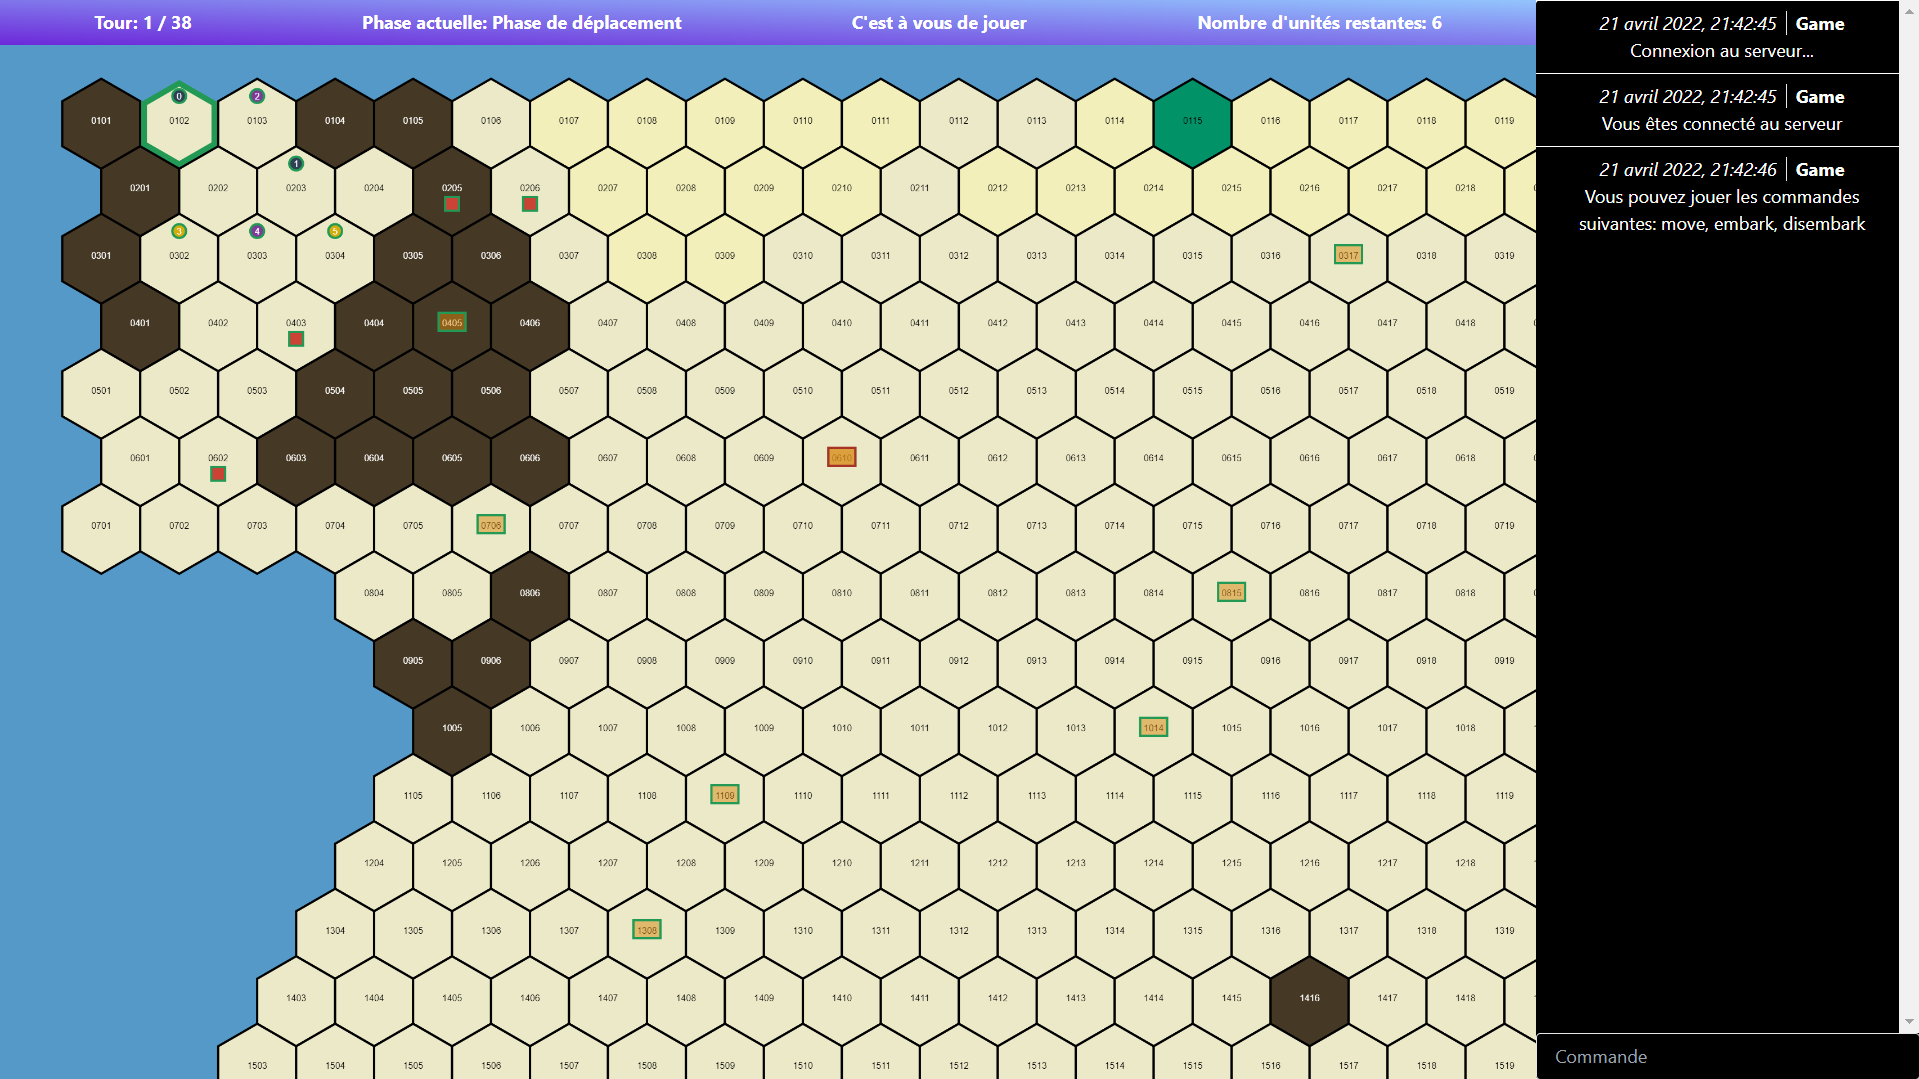
\includegraphics[scale=0.35]{data/plateau_du_jeu.png}
    \caption{Plateau du jeu Desert Fox}.
\end{figure}

En bas à gauche de la carte une légende(figure \ref{fig:map_legend}) explique les types de terrain et les types d'entités.\\

\begin{figure}[H]
    \centering
    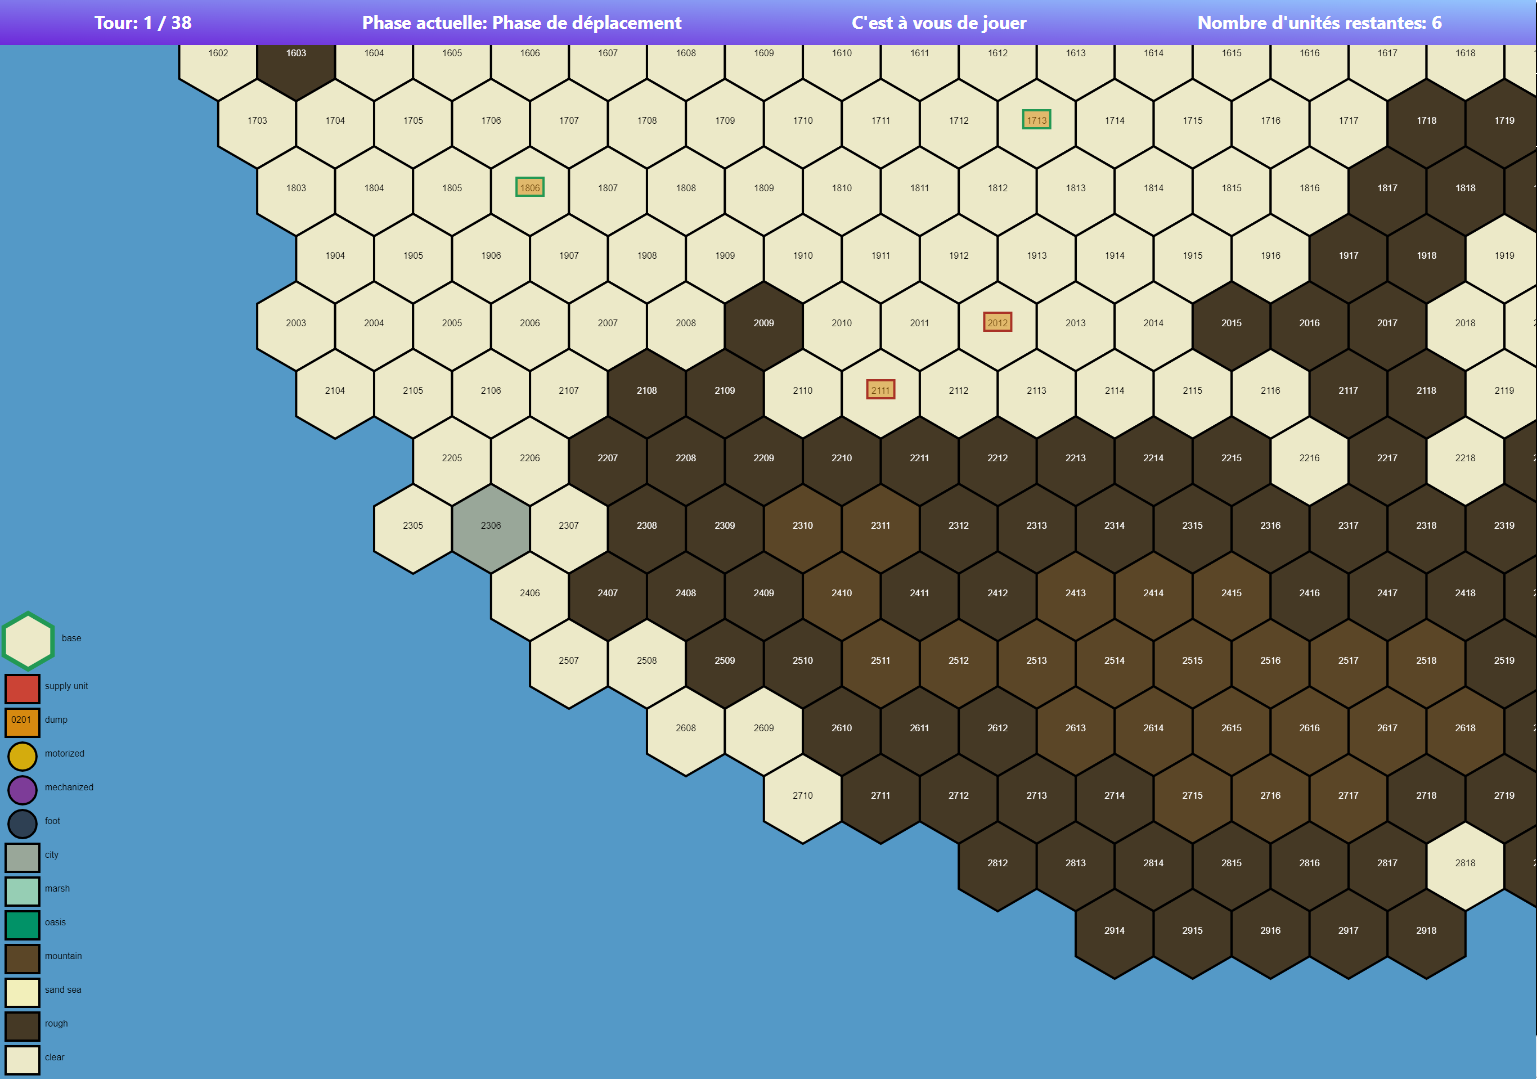
\includegraphics[scale=0.45]{data/Bas_de_map.png}
    \caption{Bas de la carte du jeu}.
\end{figure}


Voici la page du joueur 1 qui peut jouer.\\
\begin{figure}[H]
    \centering
    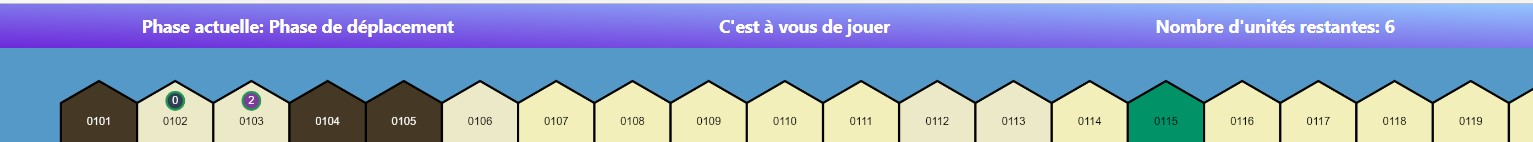
\includegraphics[scale=0.6]{data/player_1_acces.jpg}
    \caption{Barre d'information du joueur 1}.
\end{figure}

Voici la page du joueur 2 qui doit attendre l'adversaire de jouer.\\
\begin{figure}[H]
    \centering
    
\includegraphics[scale=0.6]{data/joueur_2.jpg}
    \caption{Barre d'information du joueur 2}.
\end{figure}

Le joueur qui peut jouer peut faire bouger son unité dans le terminal à droite de l'image.
Nous pouvons voir que l'unité 0 s'est déplacé de l'hexagone \lstinline{0102} à \lstinline{0206}. Le déplacement est valide, car on ne dépasse pas la capacité de mouvement de l'unité (MA).\\

\begin{figure}[H]
    \centering
    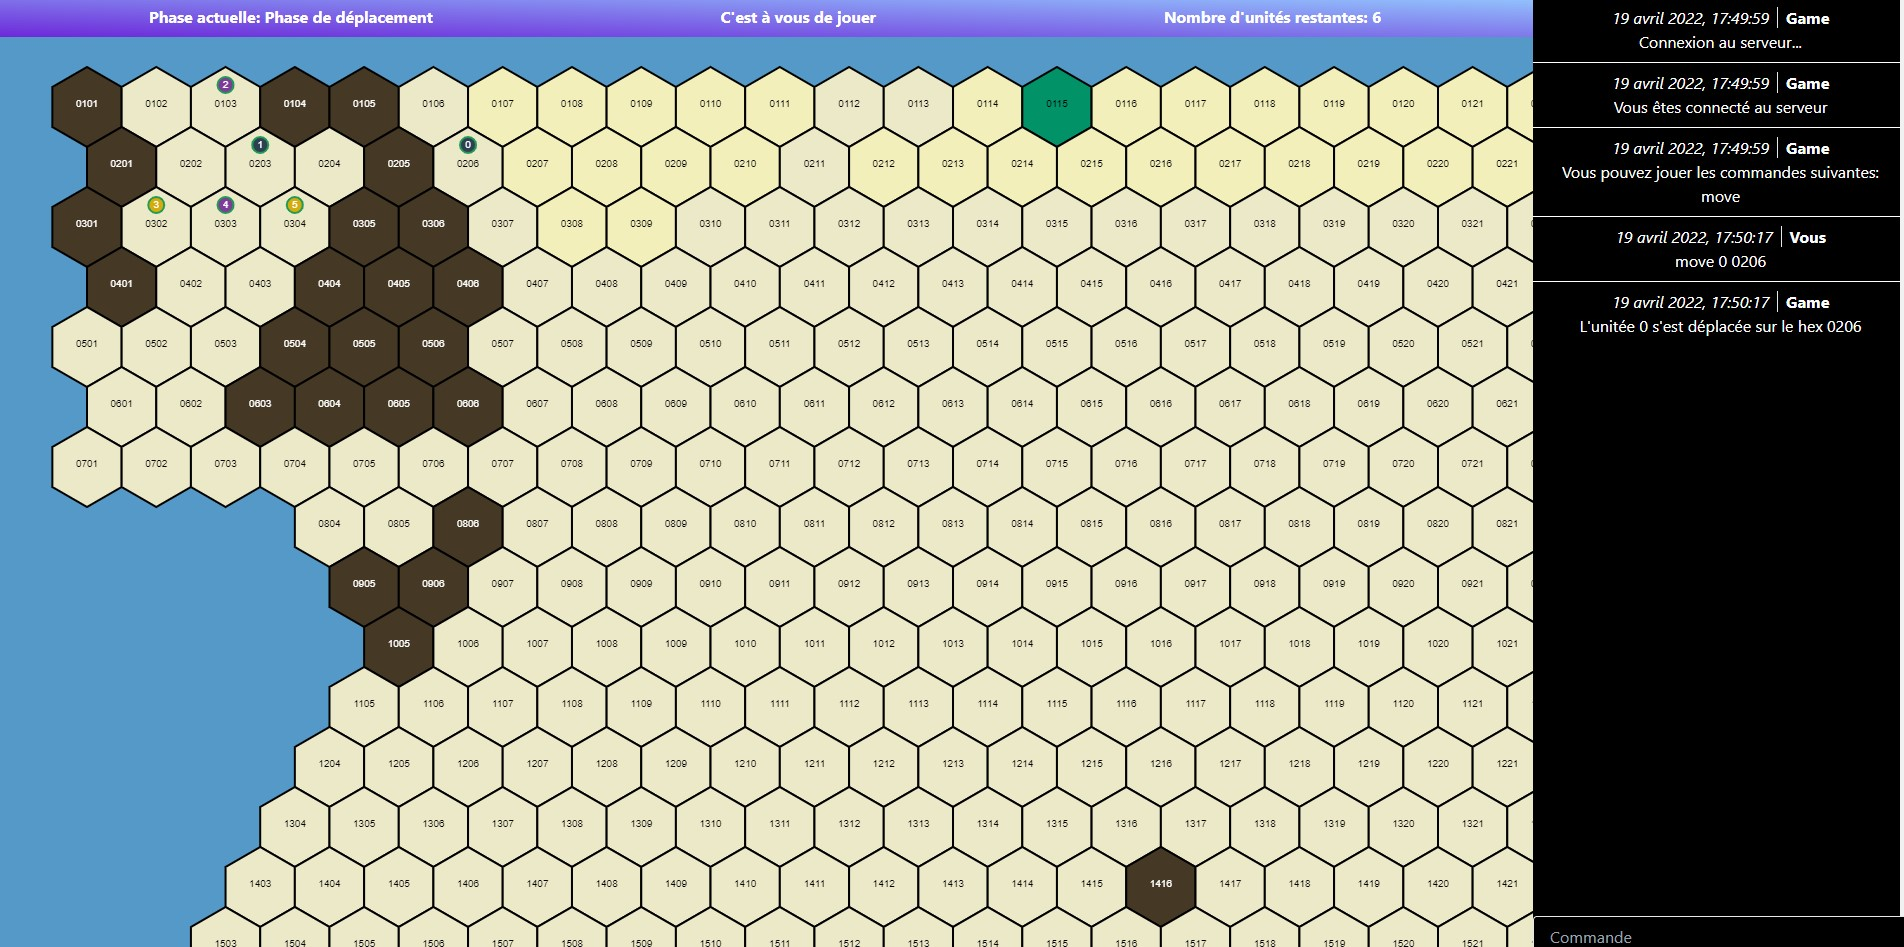
\includegraphics[scale=0.45]{data/move_unit_player_1.jpg}
    \caption{Mouvement de l'unité \lstinline{0} vers l'hexagone \lstinline{0206}}.
\end{figure}

Le joueur peut aussi utiliser une de ses unités de soutien pour bouger soit une unité de type {\tt foot} soit un dump.
Il peut faire cela avec la commande {\tt embark} qui prend en paramètre l'identifiant de l'unité du soutien qui va embarquer, ainsi que l'identifiant de l'unité qui va etre embarquée. Voici un exemple :\\

\begin{figure}[H]
    \centering
    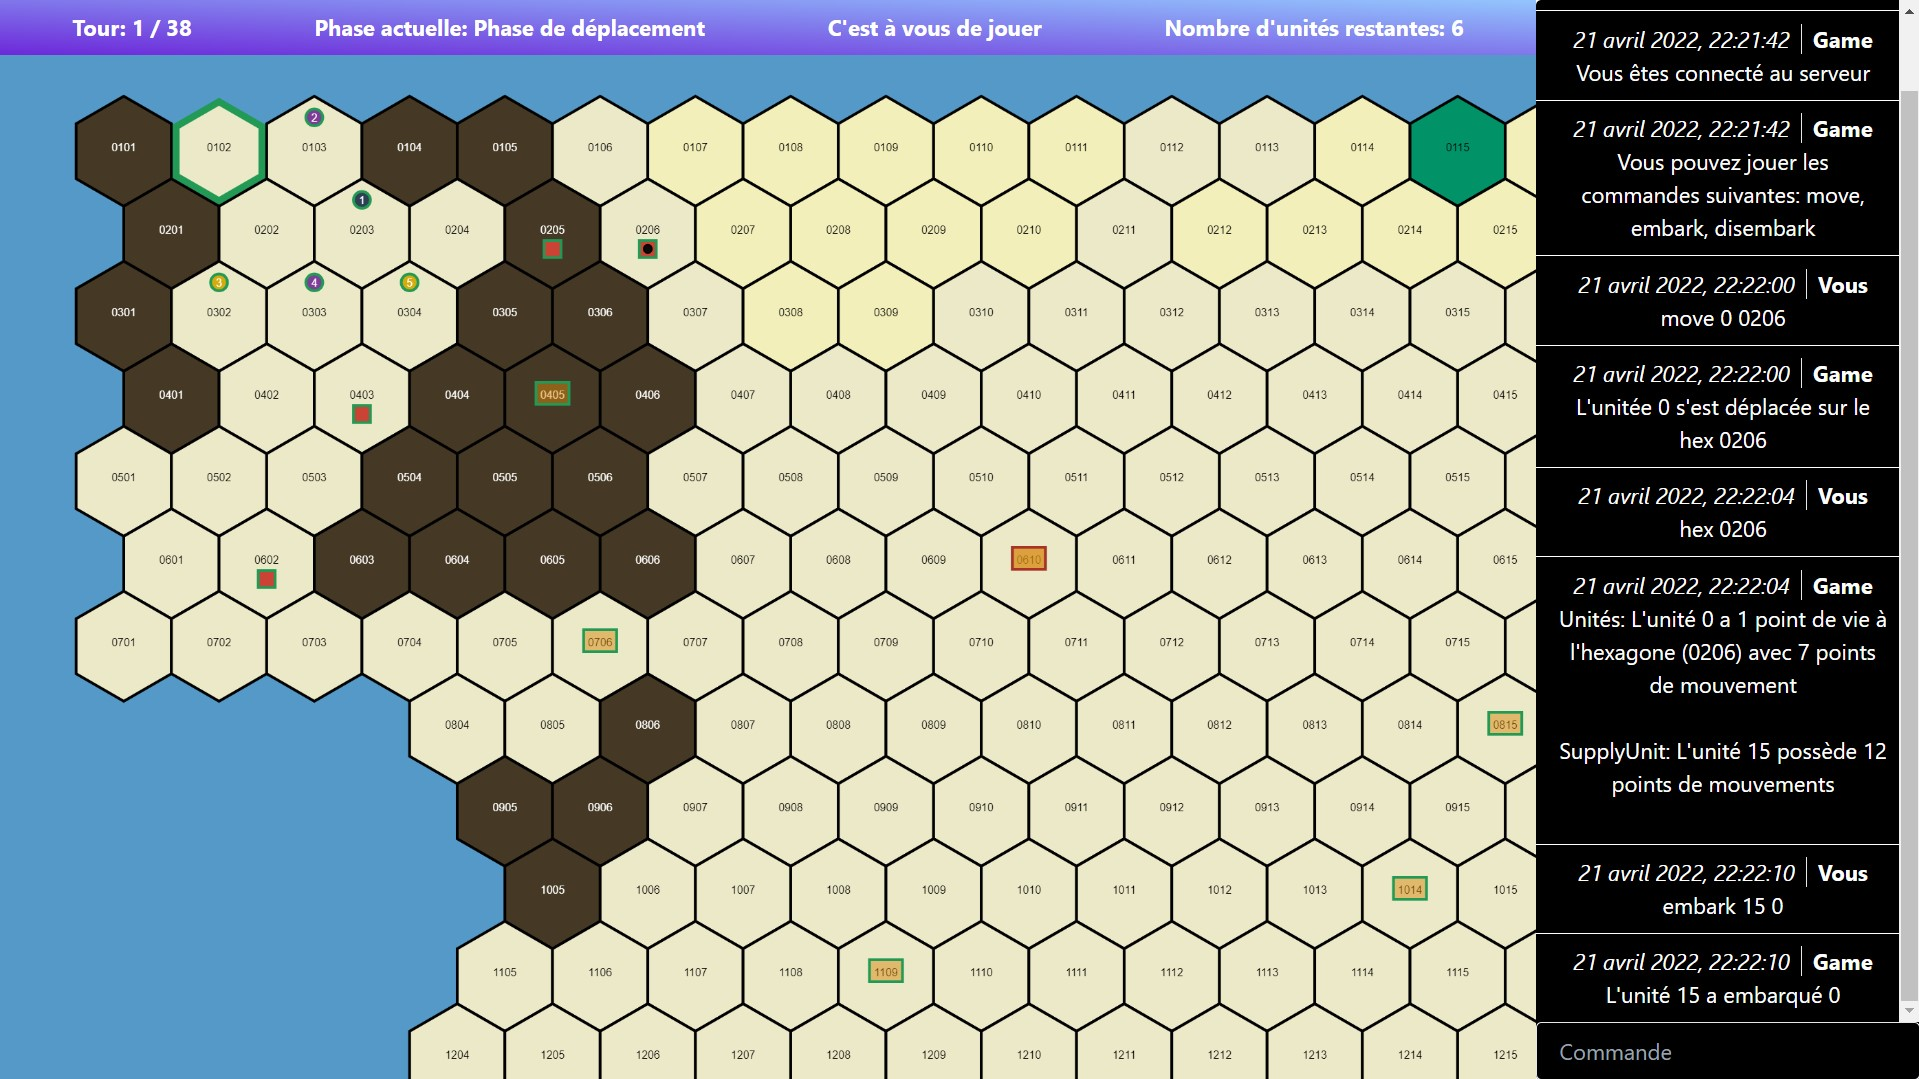
\includegraphics[scale=0.35]{data/Embark_command.jpg}
    \caption{Embarquement de l'unité \lstinline{0} dans l'unité de soutien  \lstinline{15}}.
\end{figure}

Il faut noter que l'unité qui est embarqué est inexistante dans la carte. Elle ne peut donc pas bouger elle meme, ni attaquer. Si l'unité du soutien a embarqué une unité, elle bougera avec elle. Dans la figure ci-dessous nous pouvons voir que si nous embarquons un dump, qui est une entité qui ne peut pas bouger elle meme, nous pouvons la faire bouger avec l'unité de soutien. Ici nous la bougeons de l'hexagone \lstinline{0406} vers l'hexagone \lstinline{0407} \\

\begin{figure}[H]
    \centering
    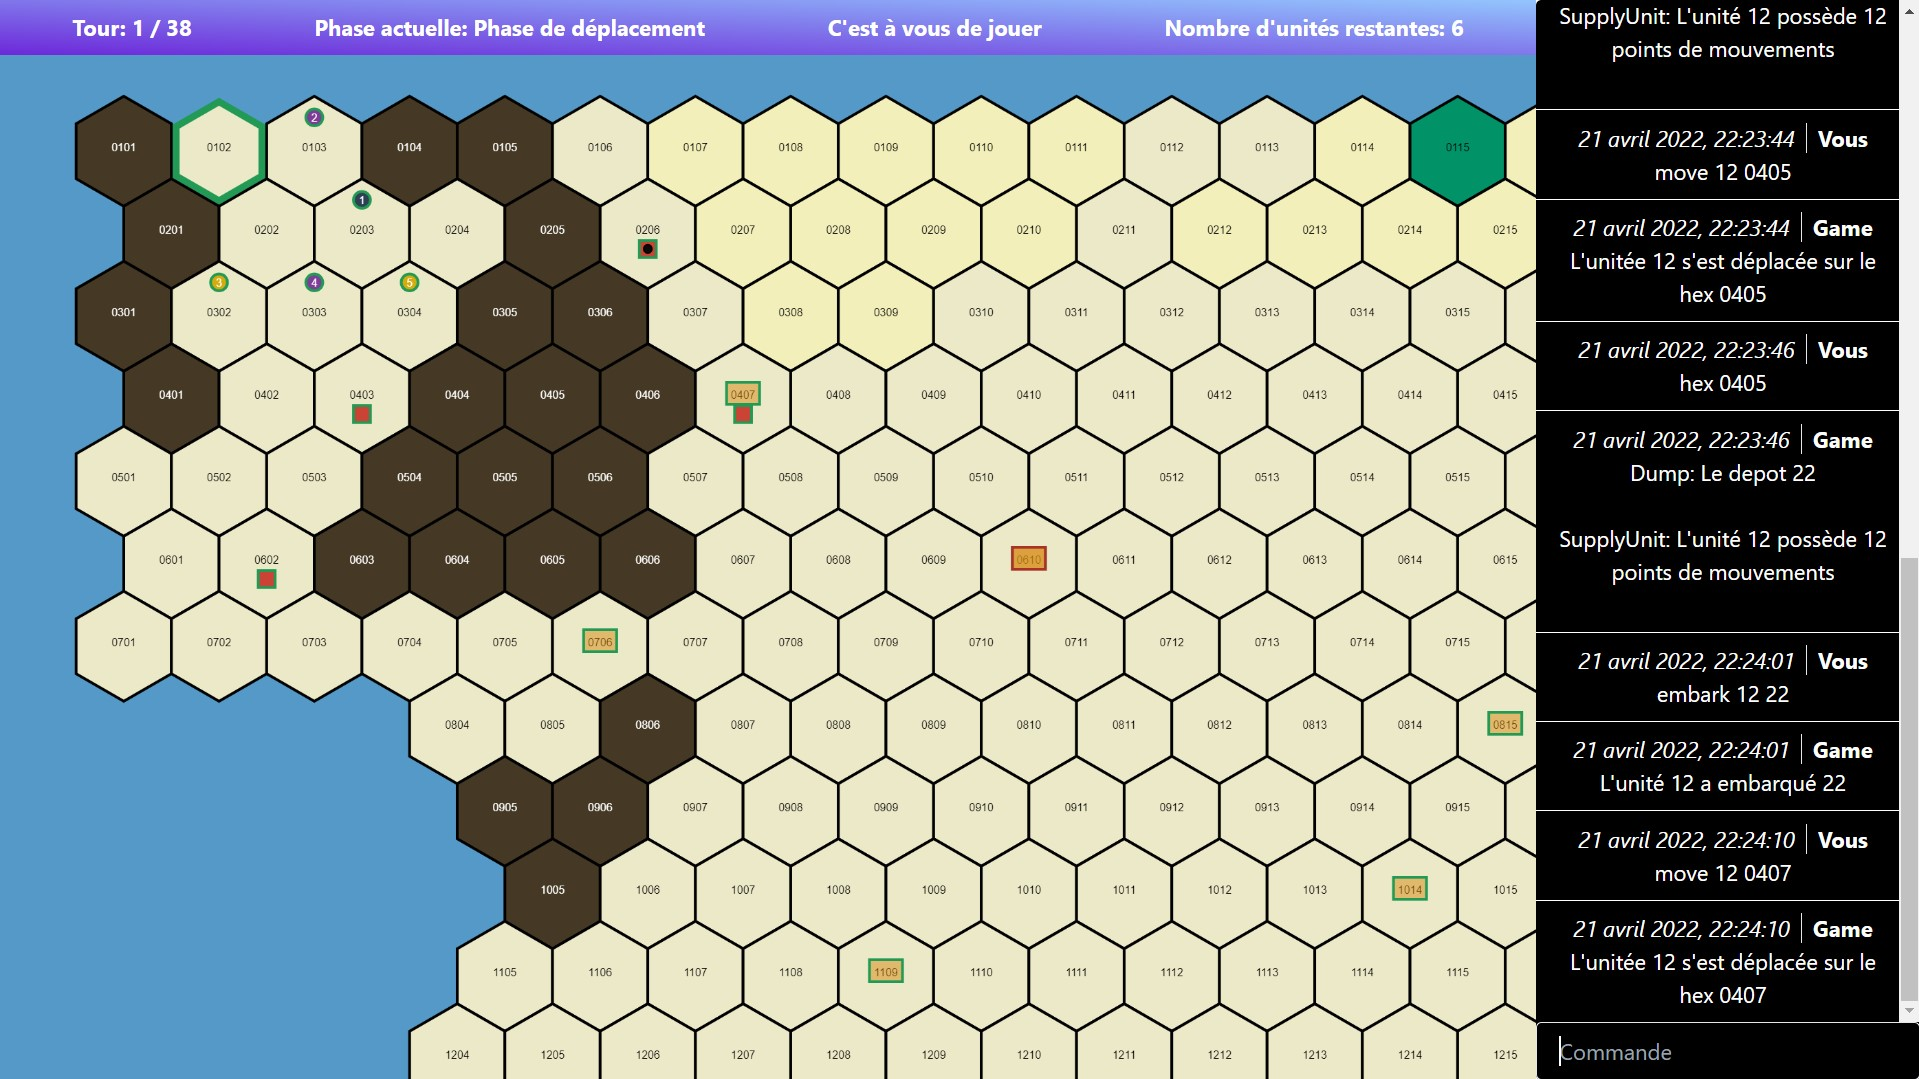
\includegraphics[scale=0.35]{data/Embark_dump.jpg}
    \caption{Embarquement du dump \lstinline{22} dans l'unité de soutien  \lstinline{12} suivi par un deplacement de l'unité du soutien à l'hexagone \lstinline{0407} (avec le dump)}.
\end{figure}

Afin de pouvoir reutiliser l'unité ou l'entité embarquée, nous devons utiliser la commande disembark, laquelle permet de debarquer cette dernière.
Dans la figure ci dessous nous pouvons voir que après avoir bougé l'unité de soutien {\tt 15}, laquelle contient l'unité {\tt 0} et désembarquer, l'unité est dorénavant disponible pour un autre mouvement ou action. Elle est aussi affichée à nouveau dans la carte.\\

\begin{figure}[H]
    \centering
    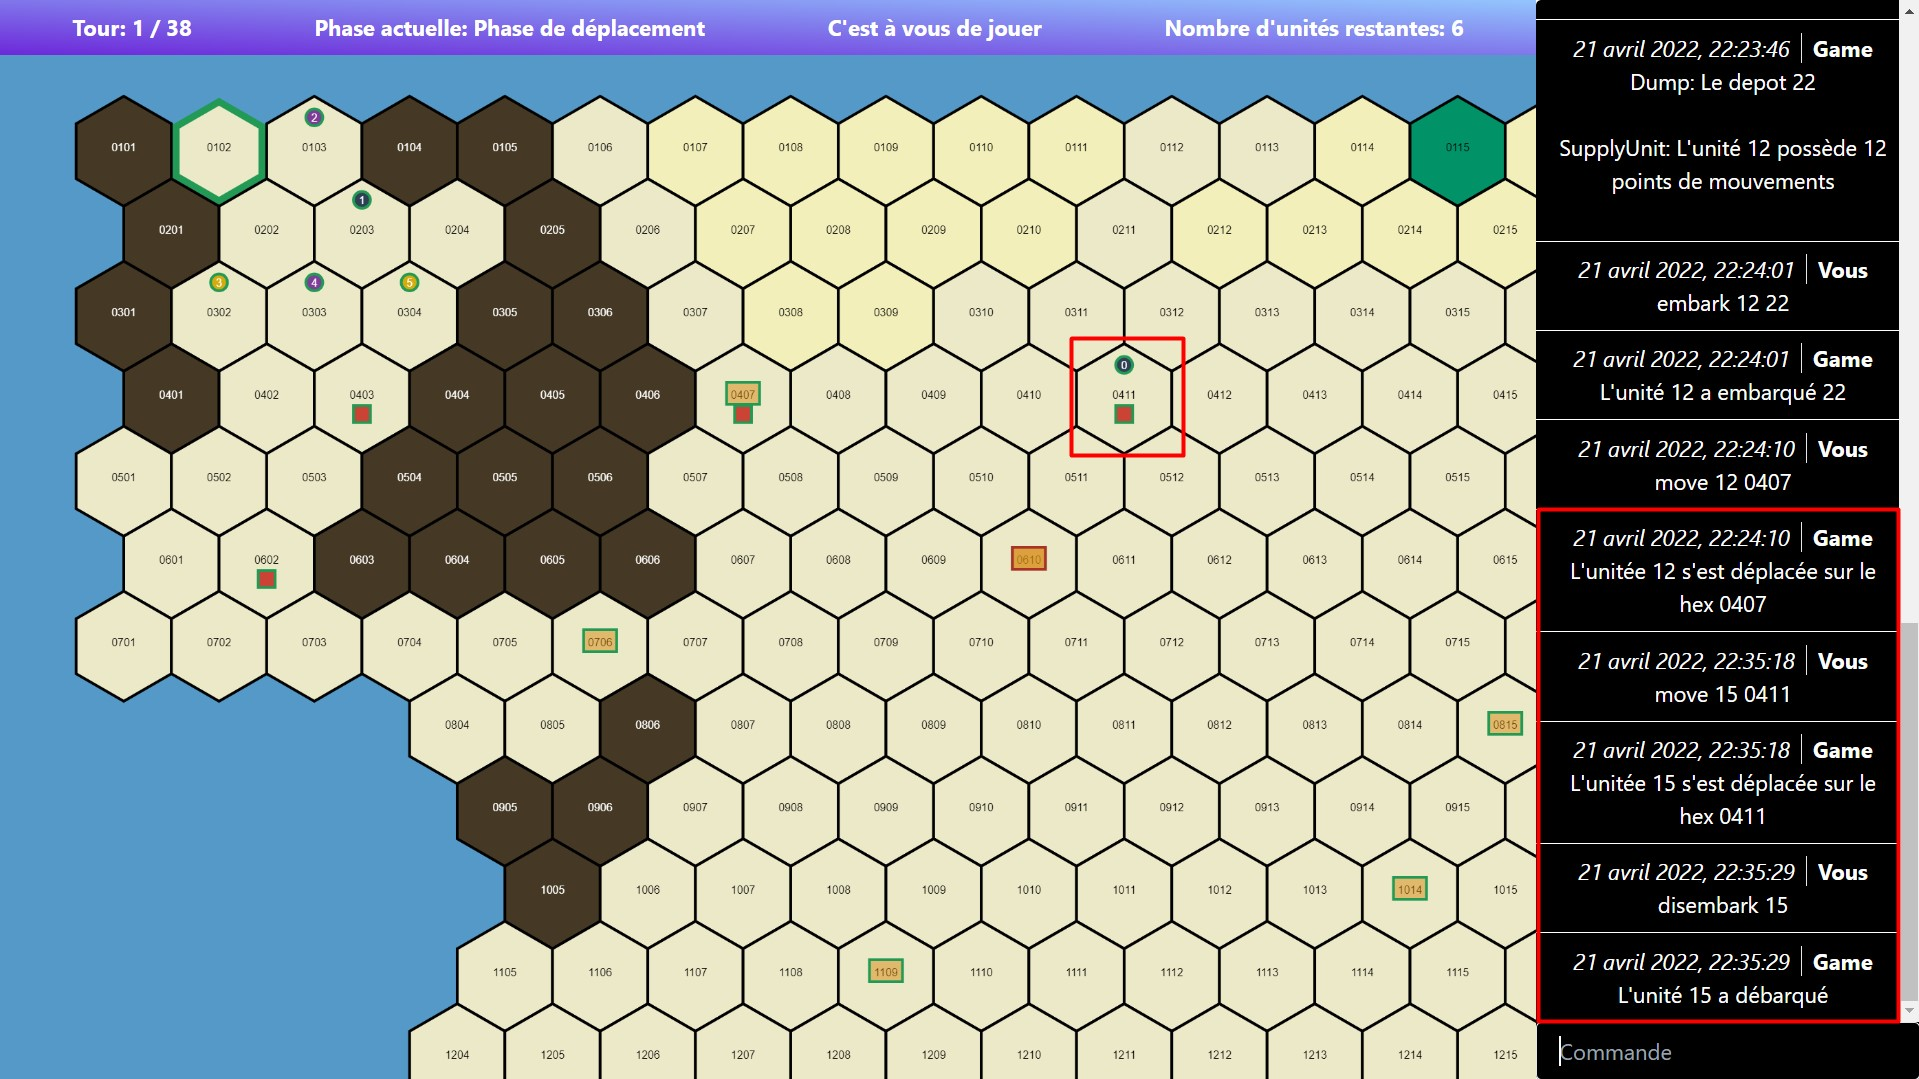
\includegraphics[scale=0.35]{data/Disembark.jpg}
    \caption{Mouvement de l'unité du soutien \lstinline{15}, laquelle contient l'unité \lstinline{0} à l'hexagone \lstinline{0411}, suivi du désembarquement de l'unité embarquée}.
\end{figure}

L'utilisateur peut aussi utiliser la commande {\tt attack} pour attaquer une unité adverse. Il faut noter que l'attaque est uniquement possible si l'unité est dans une case adjacente de l'unité adverse. Dans la figure ci-dessous, nous pouvons voir que le deuxième joueur a décidé de se préparer pour une attaque en bougeant son unité {\tt 11} à l'hexagone adjacente de l'unité {\tt 5} de son adversaire.\\

\begin{figure}[H]
    \centering
    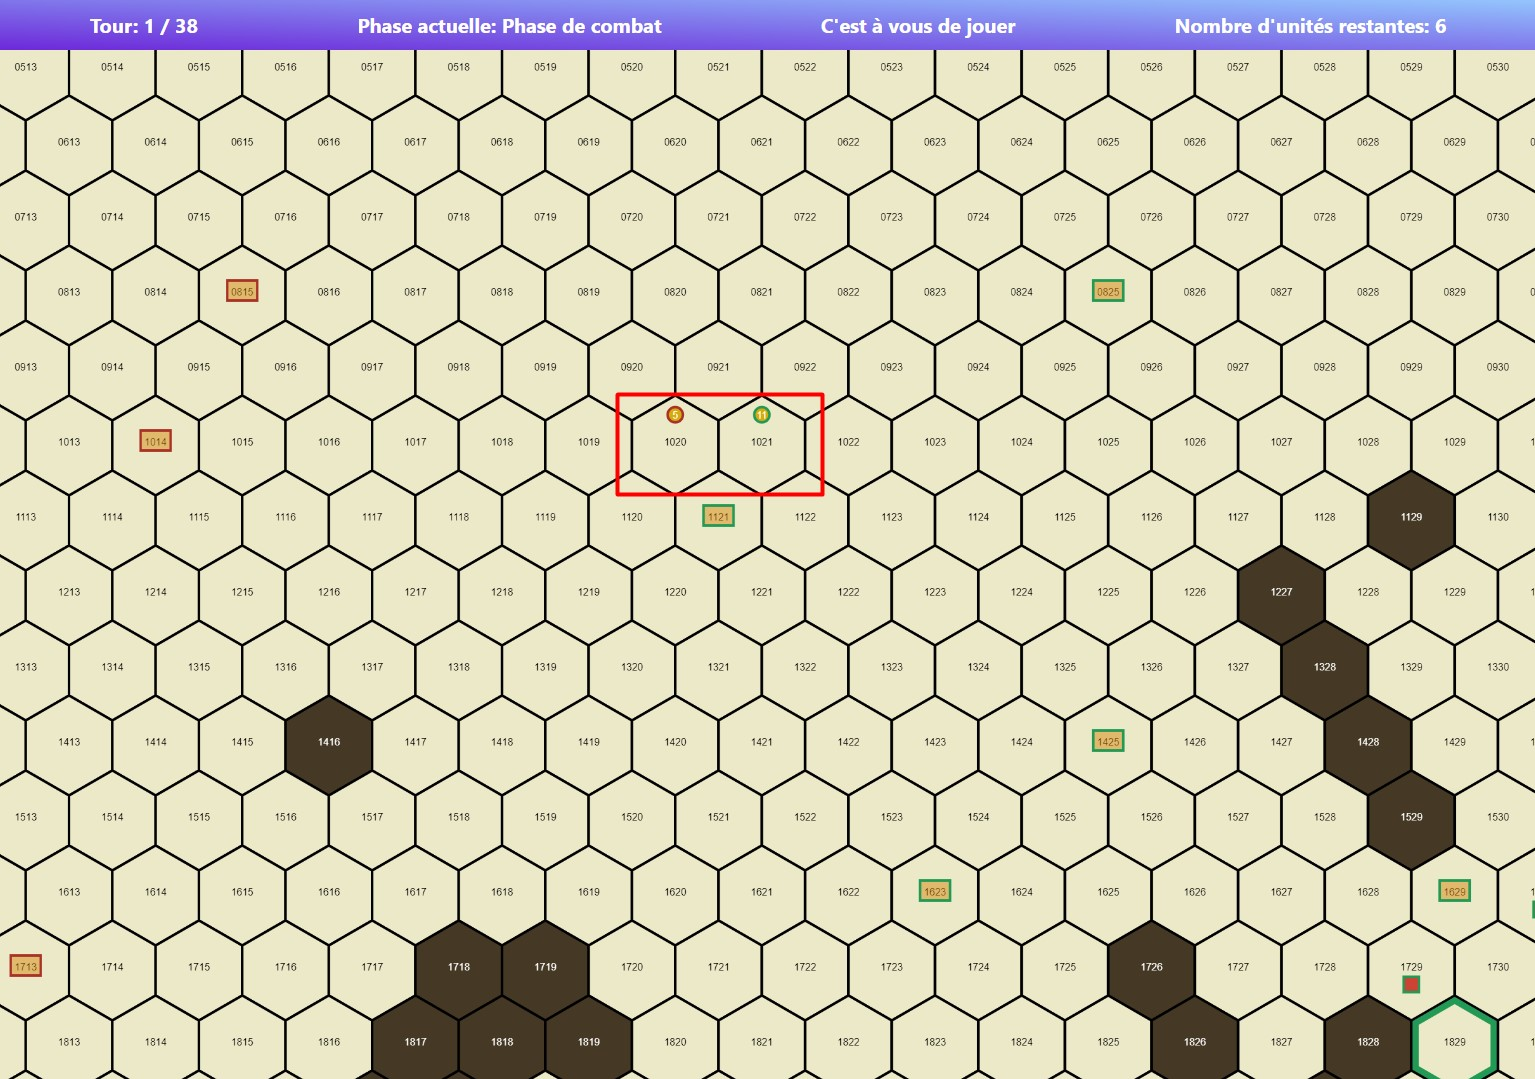
\includegraphics[scale=0.35]{data/beforeAttack.jpg}
    \caption{Mouvement de l'unité \lstinline{11} à l'hexagone \lstinline{1021}, l'hexagone adjacent à \lstinline{1020}, qui contient l'unité \lstinline{5} de l'adversaire }.
\end{figure}

Ensuite, le deuxième joueur lance l'attaque en utilisant la commande {\tt attack} suivie des deux identifiants d'hexagones ( {\tt 1021} {\tt 1020}, respectivement celle de l'attaquant et l'attaqué ). Le résultat du combat est alors affiché dans le terminal pour les deux joueurs : \\

\begin{figure}[H]
    \centering
    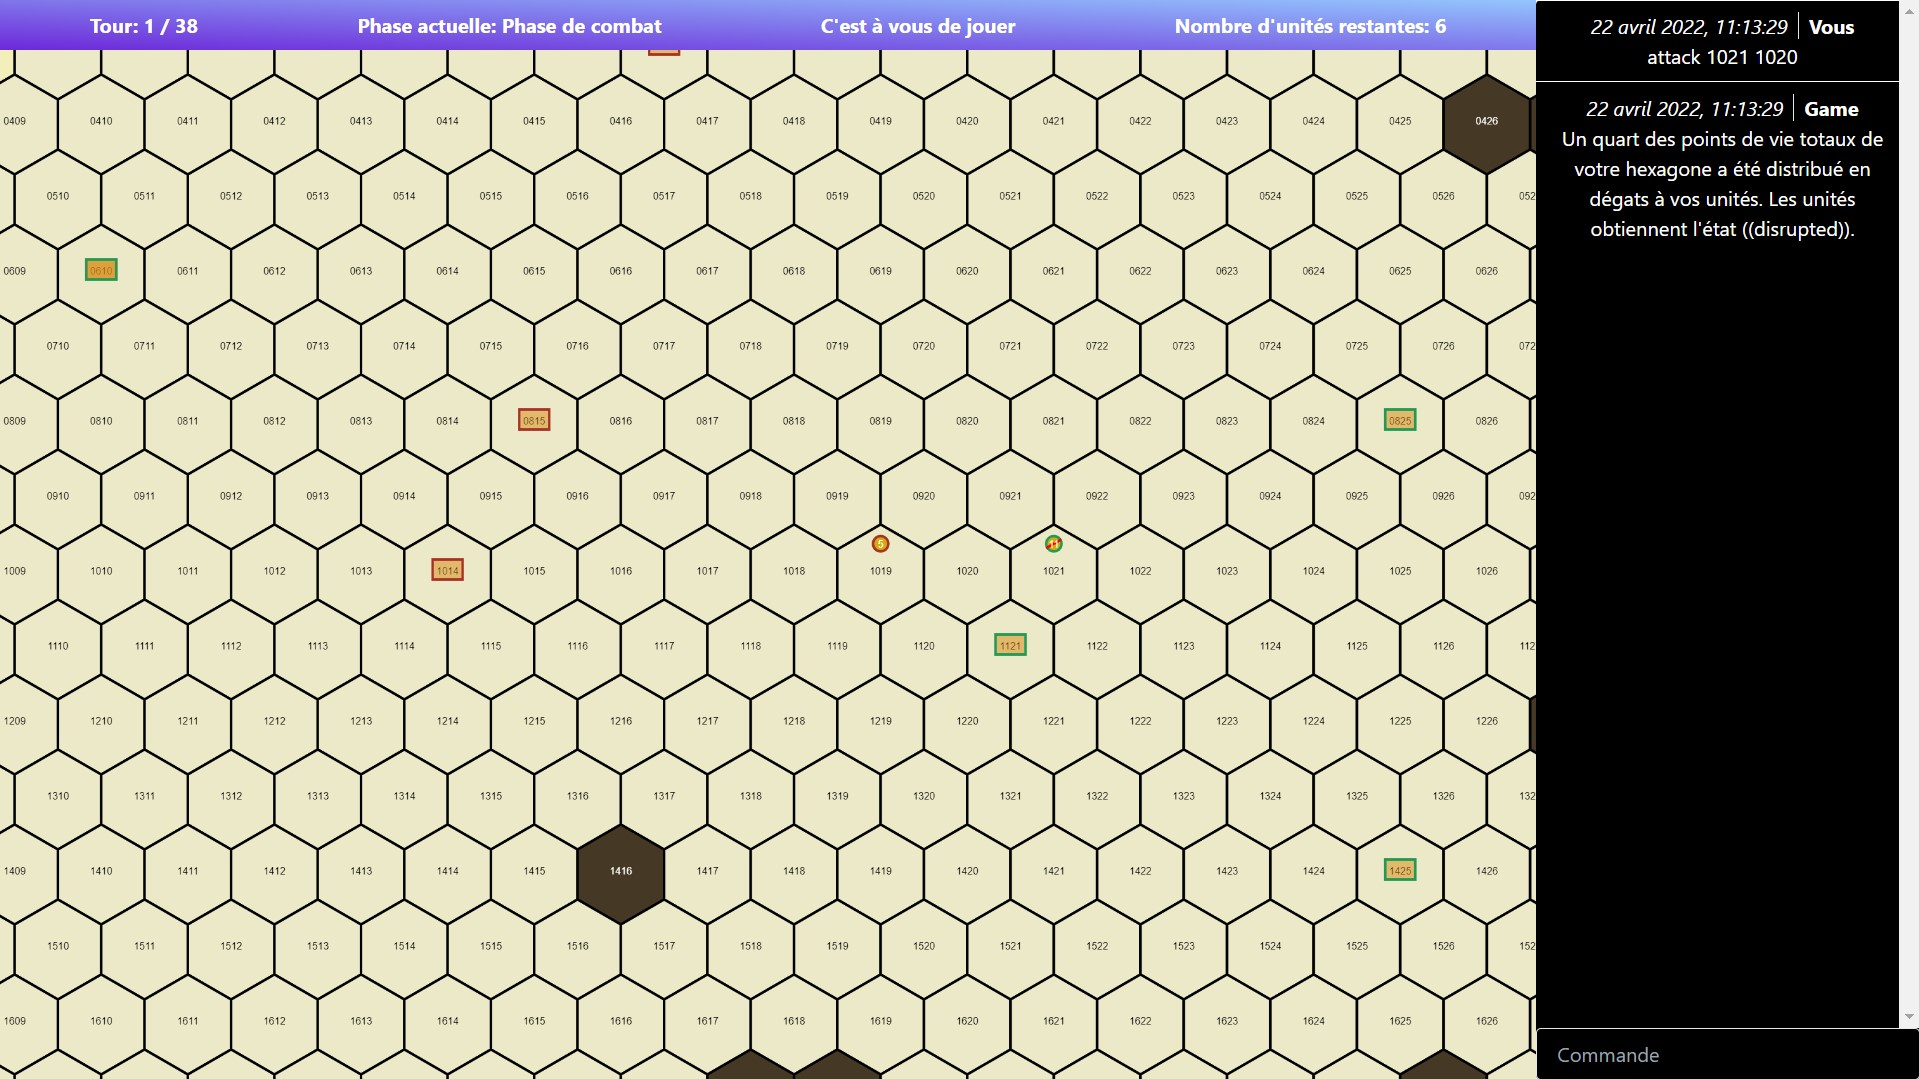
\includegraphics[scale=0.35]{data/Attacker.jpg}
    \caption{ L'exécution de la commande {\tt attack} et le résultat de cette dernière pour l'attaquant }.
\end{figure}

\begin{figure}[H]
    \centering
    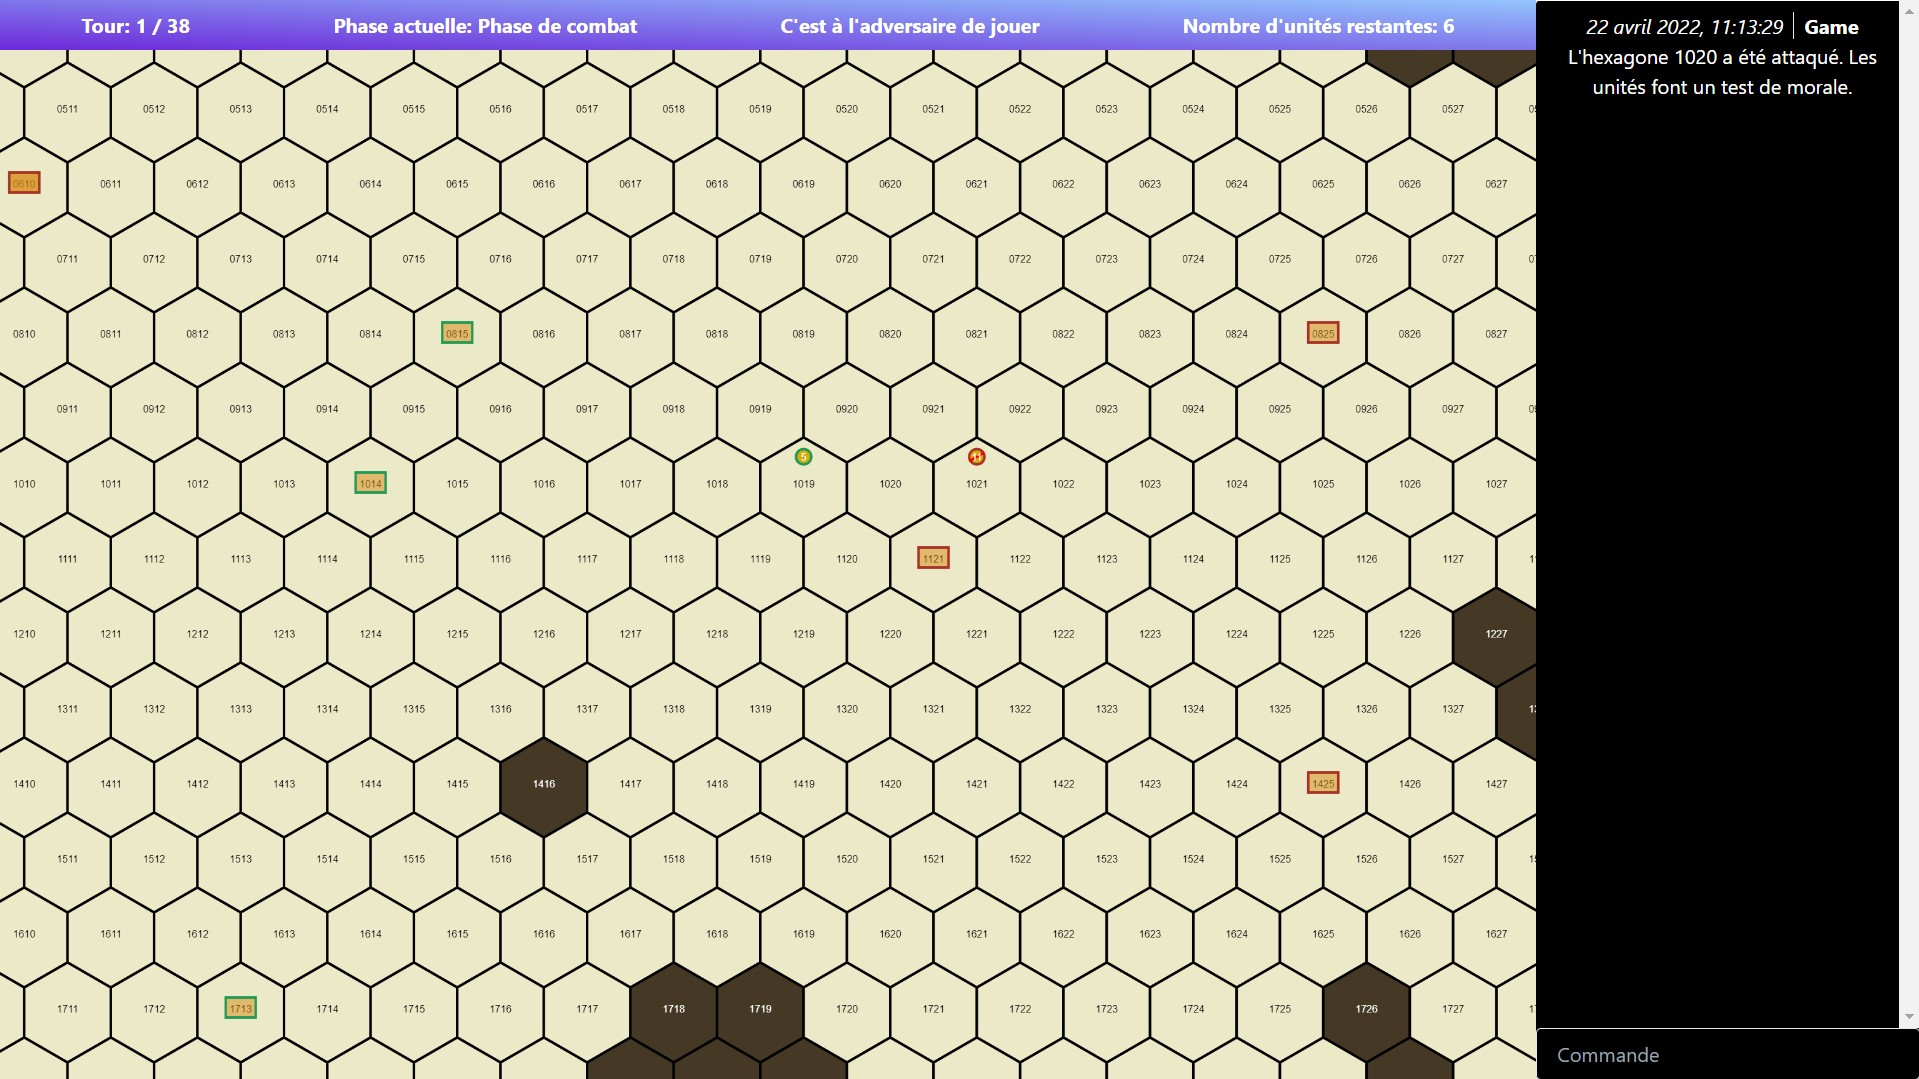
\includegraphics[scale=0.35]{data/Defender.jpg}
    \caption{L'affichage du résultat de la commande {\tt attack} pour le défendant }.
\end{figure}

Nous pouvons voir que l'attaque a échoué, et les unités attaquantes ont perdu des points de vie et sont devenues {\tt disrupted}, tandis que les unités qui défendent ont réussi à se défendre, mais font un test de morale pour vérifier si elles se replient, ce qui n'est pas arrivé dans cette situation.

Le joueur peut afficher des informations concernant ses unités dans le terminal.
En tapant \og units \fg{}, le joueur à toutes ses unités présentes avec le mouvement point et  les points de vies.
. Vous pouvez voir un exemple d'utilisation dans l'annexe a la figure \ref{fig:units_command}. \\




Quand le joueur a terminé son tour, il doit écrire dans le terminal \og done \fg{}. Le joueur ne pourra que communiquer par chat à l'adversaire et l'adversaire peuvent continuer à jouer. Voir figure \ref{fig:fin_tour}\\



Le joueur peut aussi afficher les entités, par exemple les unités, les bases, les dumps et les unités de soutien qui sont présent dans un hexagone.
Cela est possible grâce a la commande {\tt hex}, qui prend en paramètre un identifiant d'hexagone. Voir la figure \ref{fig:hex_command} pour un exemple d'utilisation.\\


Les deux joueurs peuvent communiquer ensemble  à l'aide du terminal, le joueur doit écrire au dans le terminal \og message \fg{} puis écrit son message. Voir la figure \ref{fig:message_command} pour un exemple d'utilisation. \\


Un message d'erreur s'affiche dans le terminal si le joueur effectue des mauvaises commandes.
Par exemple, le joueur oublie des arguments ou passe des mauvais arguments. Voir figure \ref{fig:wrong_command} pour un exemple d'utilisation\\

